\documentclass[10pt,a4paper]{ctexart}
\usepackage[margin=2cm]{geometry}
\usepackage{graphicx}
\usepackage{float}      % 支持 [H] 浮动体选项
\usepackage{hyperref}
\usepackage{amsmath}    % 提供方程环境
\usepackage{physics}    % 简化向量、微分算子语法
\newcommand{\myspace}[1]{\par\vspace{#1\baselineskip}} %自定义空一行
\usepackage{fancyhdr}
\pagestyle{fancy}
\fancyhf{}  % 清除所有页眉页脚
\fancyfoot[C]{\thepage}  % 在页脚中央设置页码
\renewcommand{\headrulewidth}{0pt}  % 去掉页眉横线
\renewcommand{\footrulewidth}{0pt}  % 去掉页脚横线

\usepackage{hyperref}
\hypersetup{
    colorlinks=true,
    linkcolor=blue,
    filecolor=magenta,      
    urlcolor=cyan,
    pdftitle={Overleaf Example},
    pdfpagemode=FullScreen,
    }

\usepackage{titlesec}

% 重新定义section格式
\titleformat{\section}
  {\normalfont\Large\bfseries}
  {\chinese{section}、}
  {0pt}
  {}

% 给出常用字号的自定义指令
\newcommand{\chuhao}{\fontsize{42pt}{48pt}\selectfont}
\newcommand{\xiaochu}{\fontsize{36pt}{42pt}\selectfont}
\newcommand{\xiaoer}{\fontsize{18pt}{21.6pt}\selectfont}
\newcommand{\sanhao}{\fontsize{16pt}{20pt}\selectfont}
\newcommand{\xiaosan}{\fontsize{15pt}{18pt}\selectfont}
\newcommand{\sihao}{\fontsize{14pt}{18pt}\selectfont}
\newcommand{\xiaosi}{\fontsize{12pt}{16pt}\selectfont}
\newcommand{\wuhao}{\fontsize{10.5pt}{12.6pt}\selectfont}

% 定义中文数字转换
\titleformat{\section}
  {\normalfont\Large\bfseries}
  {\zhnum{section}、}  % 使用\zhnum而不是\chinese
  {0pt}
  {}

% 标题设置
\title{\xiaochu\textbf{物理实验报告}}
\author{}
\date{}

\begin{document}

\vspace*{36pt} % 顶部空白

% 居中填写区域
\begin{center}
    
\includegraphics[width = 9cm]{figure/head.png}
    
    \xiaochu\textbf{物理实验报告}
    % 预留空白区域
    \vspace{13pt}
    \vspace{13pt}
    \vspace{13pt}
    \vspace{13pt}
    
    \sanhao\textbf{实验名称：\underline{\makebox[10cm]{ 用霍尔法测直流圆线圈与亥姆霍兹线圈磁场}}} \\[10pt]
    \sanhao\textbf{实验桌号：\underline{\makebox[10cm]{ 9}}} \\[10pt]
    \sanhao\textbf{指导教师：\underline{\makebox[10cm]{ 朱韵嫱 }}} \\[30pt]
    
    % 预留空白区域
    \myspace{6}
    
   \sihao\textbf{班级：\underline{\makebox[6cm]{}}} \\[10pt]
    \sihao\textbf{姓名：\underline{\makebox[6cm]{}}} \\[10pt]
    \sihao\textbf{学号：\underline{\makebox[6cm]{}}} \\[30pt]
    
   \sihao\textbf{实验日期: 
   \underline{\makebox[0.8cm]{2025}}  年 
   \underline{\makebox[0.4cm]{10}}月
   \underline{\makebox[0.4cm]{22}}日  
   星期\underline{\makebox[0.6cm]{三}}上午}
    
    \vspace{18pt}
    \sihao 浙江大学物理实验教学中心
    
\end{center}

\newpage

\section{预习报告}

    \subsection{实验综述}
    
    \xiaosi （自述实验现象、实验原理和实验方法，不超过300字，5分）

 本实验采用霍尔效应法测量磁场分布。
实验原理基于霍尔效应公式$B = \frac{V_H}{K_H I_s}$，
其中$K_H$为霍尔元件灵敏度，$I_s$为工作电流。
实验分为三部分：

(1)首先使用指南针确定地磁场方向，调节电流为零时记录特斯拉计读数作为地磁场本底值。

(2)测量单个载流圆线圈轴线上的磁感应强度分布，绘制B-x曲线；

(3)测量亥姆霍兹线圈轴线上的磁场分布，绘制B-x曲线，计算匀强磁场区域的理论值$B_0$，并与实测值比较计算相对误差。
    \myspace{2}
    
    
    \subsection{实验重点}
    
    \xiaosi（简述本实验的学习重点，不超过100字，3分）

    
    1. 掌握FB511型霍尔法磁场实验仪的使用方法

    2. 理解霍尔效应原理和毕奥-萨伐尔定律

    3. 学习磁场分布的测量方法和数据处理

    4. 掌握亥姆霍兹线圈产生匀强磁场的特性

    \myspace{2}
    
    \subsection{实验难点}
    
     \xiaosi（简述本实验的实现难点，不超过100字，2分）

    1. 消除地磁场等环境磁场对测量的干扰

    2. 精确控制线圈的几何位置和方向

    3. 霍尔元件的准确定位和灵敏度校准

    4. 根据测量数据绘制精确的B-x分布曲线
\myspace{2}
\section{原始数据}

    \xiaosi （将有老师签名的“自备数据记录草稿纸”的扫描或手机拍摄图粘贴在下方，20分）
   
\begin{figure}[H]
    \centering
    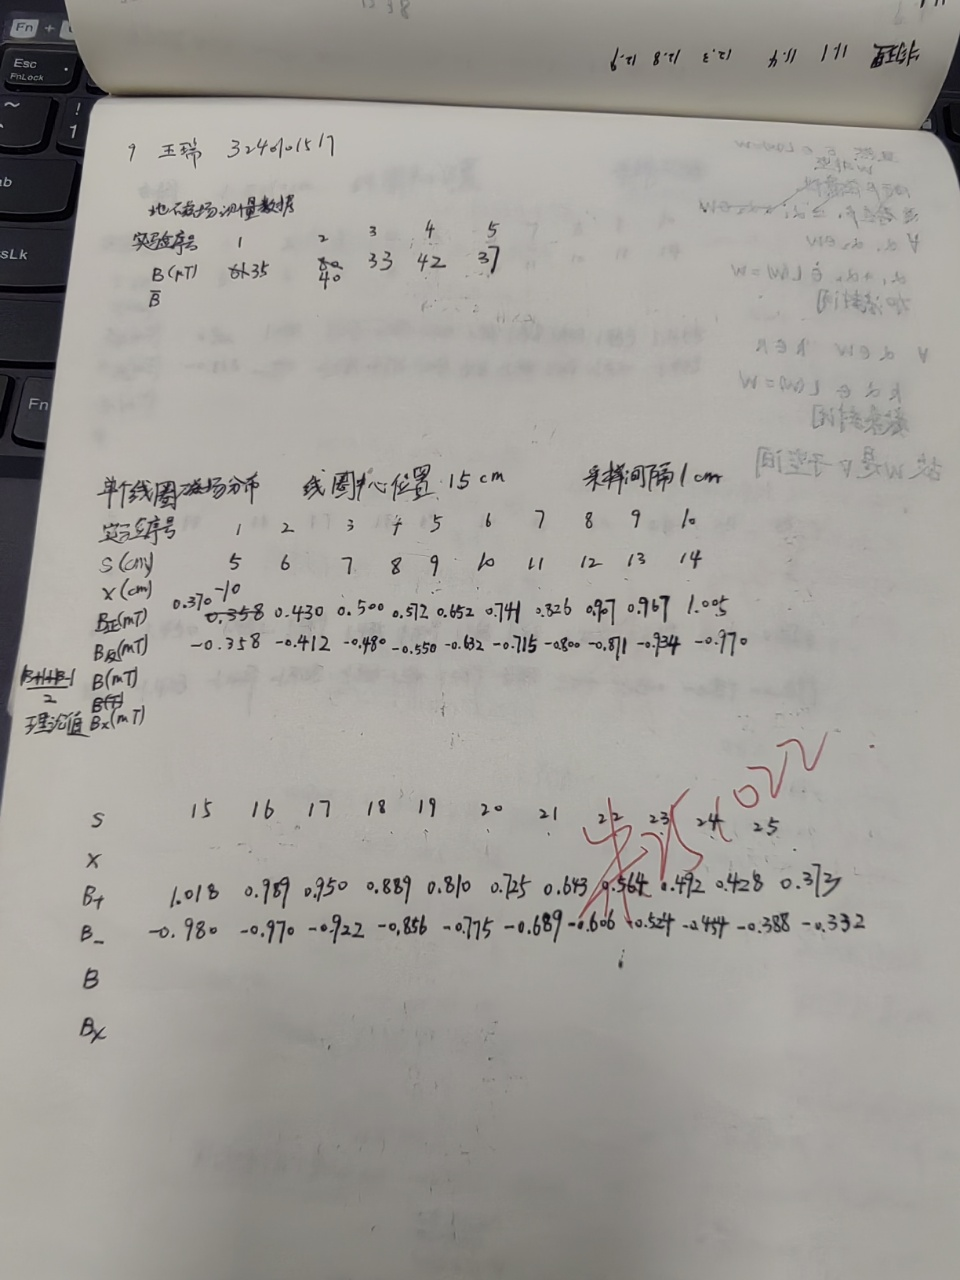
\includegraphics[width=0.8\textwidth]{figure/raw_data1.jpg}
    \caption{原始数据记录1}
\end{figure}
\begin{figure}[H]
    \centering
    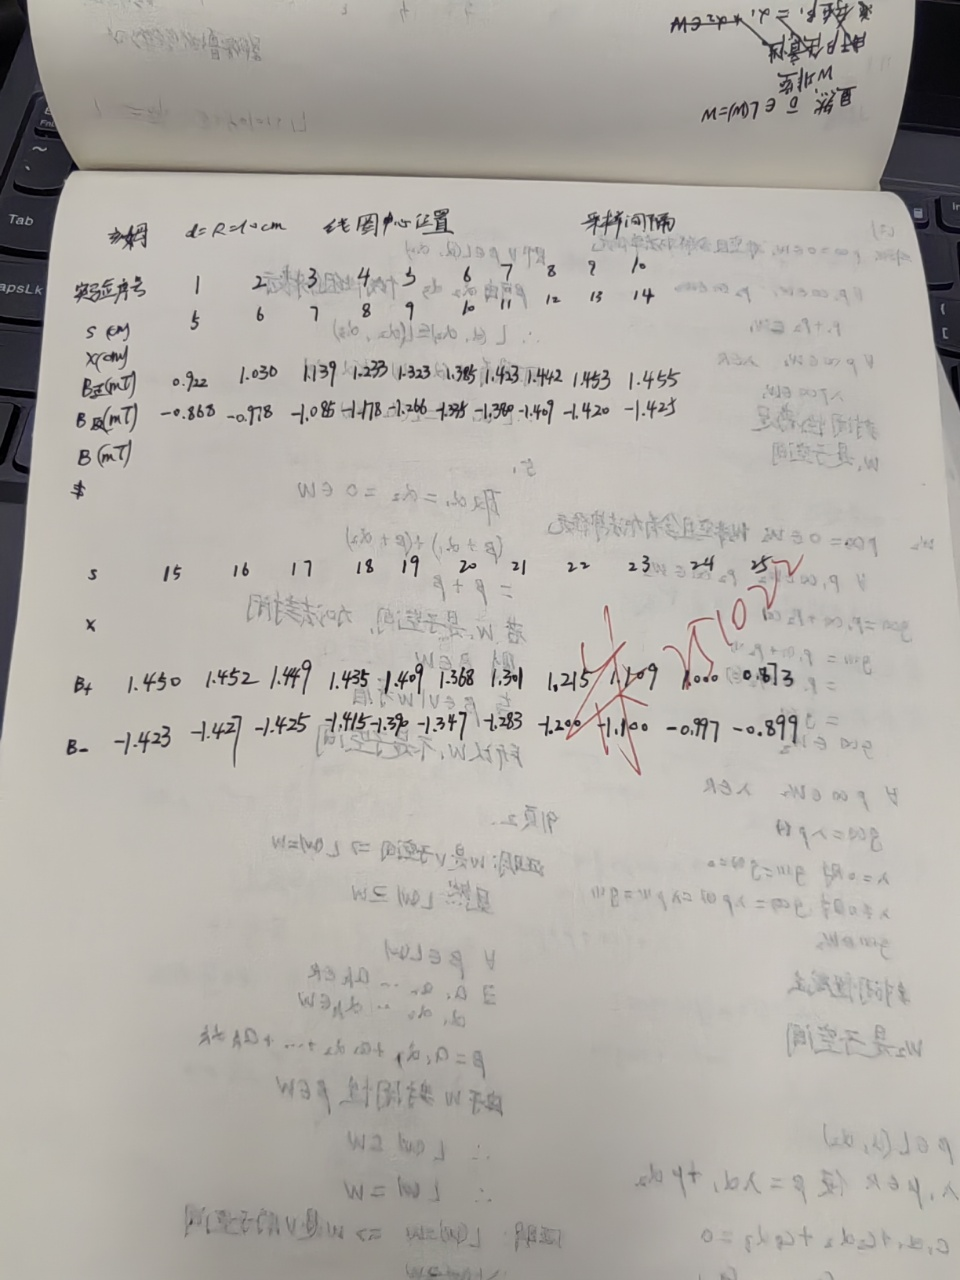
\includegraphics[width=0.8\textwidth]{figure/raw_data2.jpg}
    \caption{原始数据记录2}
\end{figure}
\section{结果与分析}

    \subsection{数据处理与结果}
    \xiaosi （列出数据表格、选择数据处理方法、给定测量或计算结果，30分）

    \subsubsection{测量地磁场}
    地磁场测量数据如下表所示：
    \begin{table}[H]
        \centering
        \begin{tabular}{|c|c|c|c|c|c|}
            \hline
            实验序号 & 1 & 2 & 3 & 4 & 5  \\
            \hline
            B($\mu T$) & 35 & 40 & 33 & 42 & 37  \\
            \hline
            $\bar{B}$($\mu T$) & \multicolumn{5}{c|}{37.4}   \\
            \hline
        \end{tabular}
        \caption{地磁场测量数据}
    \end{table}
    根据测量数据，计算得到地磁场平均值为$\bar{B} = 37.4 \mu T$。
    地磁场的标准差为：
    \[\sigma = \sqrt{\frac{1}{N-1}\sum_{i=1}^{N}(B_i - \bar{B})^2} = 3.65 \mu T\]
    A类不确定度为：
    \[U_A = \frac{\sigma}{\sqrt{N}} = 1.63 \mu T\]
    因此，根据修约规则，地磁场测量结果为$B_{地磁} = (37.4 \pm 1.6) \mu T$。
    
    \subsubsection{测绘单个载流圆线圈轴线磁感应强度分布}
    实验过程中将单个载流圆线圈放置在测量位置，调节电流并记录不同位置的磁感应强度。
    电流值为0.4A，匝数400，线圈半径10cm。测量数据如下表所示：
\begin{table}[H]
\centering
\caption{Measurement data of magnetic field}
\label{tab:magnetic_field}
\begin{tabular}{|c|c|c|c|c|c|c|c|}
\hline
实验序号 & $S$ (cm) & $x$ (cm) & $B_+$ (mT) & $B_-$ (mT) & $B_{\text{测量}}$ (mT) & $B_{\text{理论}}$ (mT) & Relative Error \\
\hline
1 & 5 & -10 & 0.370 & -0.358 & 0.364 & 0.355 & 2.5\% \\
2 & 6 & -9 & 0.430 & -0.412 & 0.421 & 0.413 & 1.9\% \\
3 & 7 & -8 & 0.500 & -0.480 & 0.490 & 0.479 & 2.3\% \\
4 & 8 & -7 & 0.572 & -0.550 & 0.561 & 0.553 & 1.4\% \\
5 & 9 & -6 & 0.652 & -0.632 & 0.642 & 0.634 & 1.3\% \\
6 & 10 & -5 & 0.741 & -0.715 & 0.728 & 0.719 & 1.3\% \\
7 & 11 & -4 & 0.826 & -0.800 & 0.813 & 0.805 & 1.0\% \\
8 & 12 & -3 & 0.907 & -0.871 & 0.889 & 0.883 & 0.7\% \\
9 & 13 & -2 & 0.967 & -0.934 & 0.950 & 0.948 & 0.2\% \\
10 & 14 & -1 & 1.005 & -0.970 & 0.987 & 0.990 & 0.3\% \\
11 & 15 & 0 & 1.018 & -0.980 & 0.999 & 1.005 & 0.6\% \\
12 & 16 & 1 & 0.989 & -0.970 & 0.980 & 0.990 & 1.0\% \\
13 & 17 & 2 & 0.950 & -0.922 & 0.936 & 0.948 & 1.3\% \\
14 & 18 & 3 & 0.889 & -0.856 & 0.872 & 0.883 & 1.2\% \\
15 & 19 & 4 & 0.810 & -0.775 & 0.792 & 0.805 & 1.6\% \\
16 & 20 & 5 & 0.725 & -0.689 & 0.707 & 0.719 & 1.7\% \\
17 & 21 & 6 & 0.643 & -0.606 & 0.624 & 0.634 & 1.6\% \\
18 & 22 & 7 & 0.564 & -0.524 & 0.544 & 0.553 & 1.6\% \\
19 & 23 & 8 & 0.492 & -0.454 & 0.473 & 0.479 & 1.3\% \\
20 & 24 & 9 & 0.428 & -0.388 & 0.408 & 0.413 & 1.2\% \\
21 & 25 & 10 & 0.373 & -0.332 & 0.353 & 0.355 & 0.6\% \\
\hline
\end{tabular}
\end{table}
    绘制的B-x分布曲线如下图所示：
    \begin{figure}[H]
        \centering
        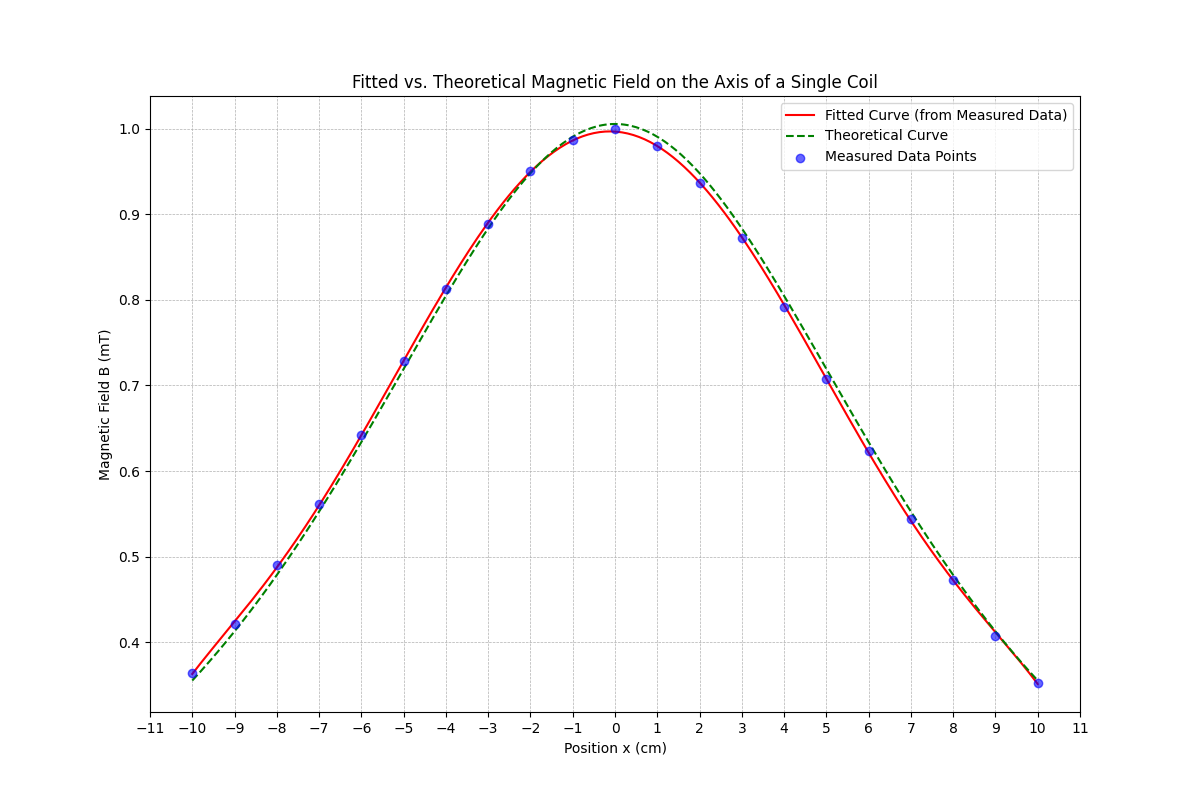
\includegraphics[width=0.8\textwidth]{figure/single.png}
        \caption{单个载流圆线圈轴线磁感应强度分布曲线}
    \end{figure}
可以看到，实验测量值和理论值误差较小，大部分在2\%以内，说明实验结果较为准确。
从图像上也可以看出，测量图像和理论图像基本重合，表明实验结果误差不大。

曲线在x=0cm处取得最大值，呈现轴对称分布，符合载流圆线圈轴线磁场分布的理论预期。在x=0两侧B值逐渐减小。


    \subsubsection{测绘亥姆霍兹线圈轴线磁感应强度分布}
    实验过程中将亥姆霍兹线圈放置在测量位置，调节电流并记录不同位置的磁感应强度。
    电流值为0.4A，匝数400，线圈半径10cm。线圈1位于S=10cm处，线圈2位于S=20cm处。测量数据如下表所示：
    \begin{table}[H]
\centering
\caption{Magnetic field measurement data}
\label{tab:magnetic_field}
\begin{tabular}{|c|c|c|c|c|c|}
\hline
实验序号 & $S$ (cm) & $x$ (cm) & $B_+$ (mT) & $B_-$ (mT) & $B_{\text{测量}}$ (mT) \\
\hline
1 & 5 & -10 & 0.922 & -0.868 & 0.895 \\
2 & 6 & -9 & 1.030 & -0.978 & 1.004 \\
3 & 7 & -8 & 1.139 & -1.085 & 1.112 \\
4 & 8 & -7 & 1.233 & -1.178 & 1.206 \\
5 & 9 & -6 & 1.323 & -1.266 & 1.294 \\
6 & 10 & -5 & 1.385 & -1.335 & 1.360 \\
7 & 11 & -4 & 1.423 & -1.380 & 1.401 \\
8 & 12 & -3 & 1.442 & -1.409 & 1.425 \\
9 & 13 & -2 & 1.453 & -1.420 & 1.437 \\
10 & 14 & -1 & 1.455 & -1.425 & 1.440 \\
11 & 15 & 0 & 1.450 & -1.423 & 1.437 \\
12 & 16 & 1 & 1.452 & -1.427 & 1.440 \\
13 & 17 & 2 & 1.449 & -1.425 & 1.437 \\
14 & 18 & 3 & 1.435 & -1.415 & 1.425 \\
15 & 19 & 4 & 1.409 & -1.390 & 1.399 \\
16 & 20 & 5 & 1.368 & -1.347 & 1.357 \\
17 & 21 & 6 & 1.301 & -1.283 & 1.292 \\
18 & 22 & 7 & 1.215 & -1.200 & 1.208 \\
19 & 23 & 8 & 1.109 & -1.100 & 1.105 \\
20 & 24 & 9 & 1.000 & -0.997 & 0.998 \\
21 & 25 & 10 & 0.873 & -0.899 & 0.886 \\
\hline
\end{tabular}
\end{table}
绘制B-x分布曲线如下图所示：
\begin{figure}[H]
    \centering
    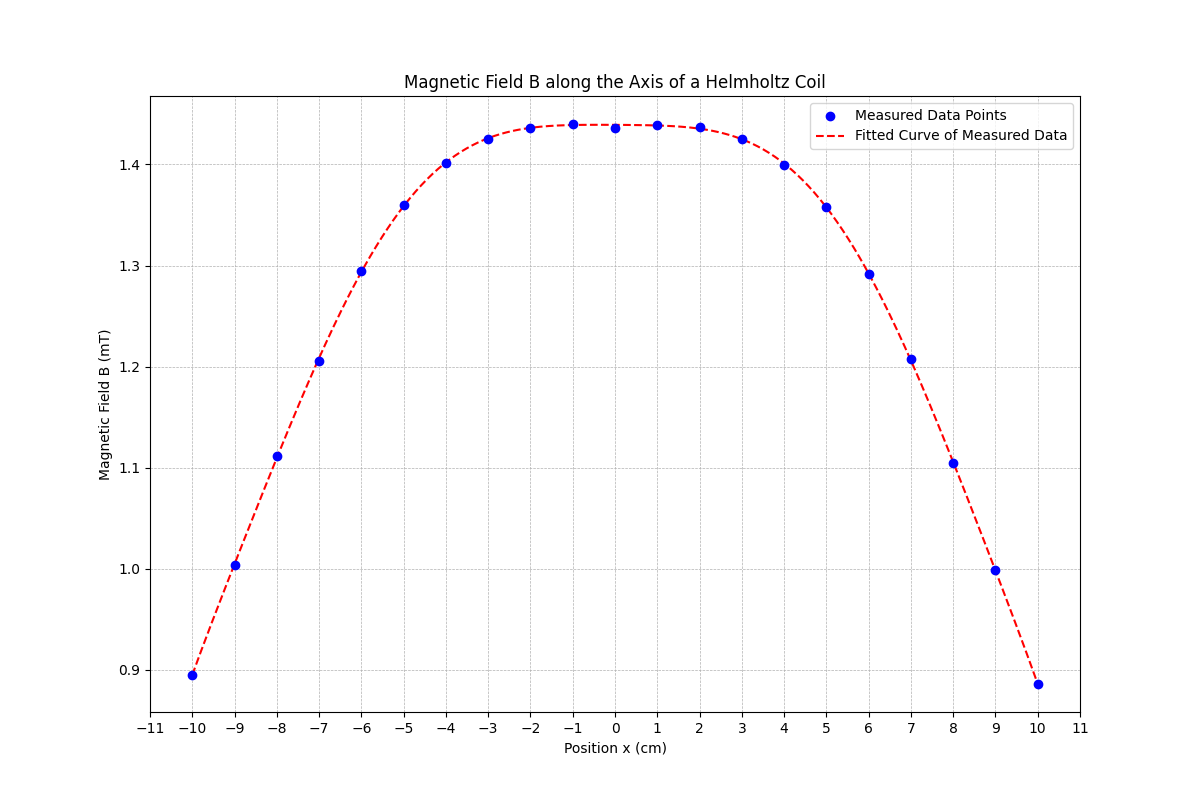
\includegraphics[width=0.8\textwidth]{figure/double.png}
    \caption{亥姆霍兹线圈轴线磁感应强度分布曲线}
\end{figure}
可以看到，在-2cm到2cm范围内，磁感应强度变化较小，形成了一个近似匀强磁场区域。其它区域随着x绝对值增大，磁感应强度逐渐减小。
根据亥姆霍兹线圈的理论公式，计算匀强磁场区域的理论值$B_0$：
\[B_0 = \frac{8\mu_0 N I}{\sqrt{125} R}\]
代入参数$N=400$，$I=0.4A$，$R=0.1m$，得到$B_0 \approx 1.439mT$。
实验测量值在匀强磁场区域内的平均值约为$1.437mT$，与理论值非常接近。计算相对误差：
\[\text{Relative Error} = \frac{|B_{\text{测量}} - B_0|}{B_0} \times 100\% \approx 0.1\%\]
实验结果表明，亥姆霍兹线圈能够在其轴线中心区域产生近似匀强磁场，且实验测量值与理论值高度一致，验证了亥姆霍兹线圈的磁场特性。
    \myspace{2}
\subsection{误差分析}
    \xiaosi （运用测量误差、相对误差、不确定度等分析实验结果，20分）

地磁场测量误差分析：

地磁场测量中，主要误差来源于仪器读数误差和环境磁场干扰。仪器读数误差可通过多次测量取平均值减小，环境磁场干扰则较难控制，可能导致测量值偏离真实地磁场值。通过计算标准差和A类不确定度，最终地磁场测量结果为$B_{地磁} = (37.4 \pm 1.6) \mu T$，相对不确定度约为4.3\%。

单个载流圆线圈磁场测量和亥姆霍兹线圈磁场测量误差分析：

两个实验的关键都是测量磁场和绘制图像。

磁场测量的误差来源：主要包括仪器精度限制、环境磁场干扰、线圈位置和电流稳定性等因素。
首先，地磁场和环境磁场的干扰难以完全消除，会影响测量精度。
其次，霍尔元件的定位可能存在偏差，特别是沿轴线方向的微小位移会导致磁场测量值的变化。
此外，仪器的读数误差也不容忽视，由于仪器老化，可能导致测量值偏差。
温度变化也可能影响霍尔元件的灵敏度，虽然实验过程中尽量保持环境温度稳定，但微小的温度波动仍可能引入误差。
最后，线圈的几何参数（如半径、匝数等）的标称值与实际值之间可能存在微小差异，这会影响理论计算结果的准确性。

绘制图像也存在误差，主要来自数据点的离散性和拟合方法选择。数据点的离散性可能导致曲线不够平滑，影响对磁场分布规律的判断。拟合方法选择不当也可能引入系统误差，导致理论与实验曲线偏离。

总体来看，单个载流圆线圈和亥姆霍兹线圈磁场测量的相对误差均在2\%以内，表明实验结果较为准确。通过改进测量方法和数据处理技术，有望进一步减小误差，提高实验精度。
    \subsection{实验探讨}
    \xiaosi （对实验内容、现象和过程的小结，不超过100字，10分）
    
通过本次实验，我们首先测量了地磁场的值，然后验证了霍尔效应测量磁场的可行性，掌握了磁场分布测量的基本方法。
实验结果表明，单个载流圆线圈的磁场分布与理论预期相符，呈现轴对称特点；亥姆霍兹线圈在中心区域确实能产生均匀磁场，测量值与理论值高度吻合（相对误差仅0.1\%）。
\section{思考题}

    \xiaosi （解答教材或讲义或老师布置的思考题，10分）
\subsection{为什么在测量直流磁场时，必须考虑地球磁场对被测磁场的影响？}
地球磁场约为50μT量级，与许多直流磁场测量目标同数量级，若不考虑其影响会导致显著误差。
可以看到测量磁场强度大约分布在0.3mT到1.4mT之间，地磁场约占测量值的2.5\%到12\%，若不扣除地磁场影响，测量结果会偏高，影响实验准确性。
\subsection{载流线圈轴线上磁场的分布规律如何？}
载流圆线圈轴线上磁场分布呈现轴对称特性，磁感应强度在中心位置达到最大值，随着距离增大逐渐减小。
\subsection{亥姆霍兹线圈是怎么组成？其基本条件有哪些？它的磁场分布特点又怎样？改变两圆线圈间距后，线圈轴线上的磁场分布情况如何？}
亥姆霍兹线圈由两个同轴平行圆线圈组成，间距等于半径（R=10cm时间距10cm）。这种结构在中心区域产生均匀磁场。若改变间距，均匀性会被破坏：间距增大时磁场不均匀度增加，间距过小均匀区域减小。
\subsection{霍尔元件放入磁场时，不同方向上的特斯拉计指示值不同，哪个方向最大？}
当霍尔元件敏感面与磁场方向垂直时特斯拉计读数最大，此时霍尔电压响应最灵敏。
\subsection{试分析载流线圈磁场分布的理论值和实验值的误差产生原因？}
误差主要来自：a) 地磁场干扰；b) 线圈几何参数偏差；c) 霍尔元件定位误差；d) 温度变化影响灵敏度；e) 测量仪器精度限制；f)电流微小波动不稳定。其中系统误差可通过正反向测量消除，随机误差需通过多次测量减小。
\newpage

\sihao\textbf{注意事项：}
\xiaosi
\begin{enumerate}
    \item 用PDF格式上传“实验报告”，文件名：学生姓名+学号+实验名称+周次。
    \item  “实验报告”必须递交在“学在浙大”的本课程的对应实验项目的“作业”模块内。
    \item  “实验报告”成绩必须在“浙江大学物理实验教学中心网站”-“选课系统”内查询。
    \item 教学评价必须在“浙江大学物理实验教学中心网站”-“选课系统”内进行，学生必须进行教学评价，才能看到实验报告成绩，教学评价必须在本次实验结束后 3 天内进行。
\end{enumerate}

\vspace{1cm}
\xiaosi\centering \textbf{浙江大学物理实验教学中心制}

\end{document}